\begin{frame}
\begin{block}{ Week 1 - L2: System Architecture }
Welcome 
\end{block}
\end{frame}



\begin{frame}
\begin{block}{System Architecture Modeling}
Architecture models that describe the functional, logical, and physical architectures of the system. 
\end{block}
\end{frame}


\begin{frame}
\frametitle{Schematics Representation  }
\begin{figure}
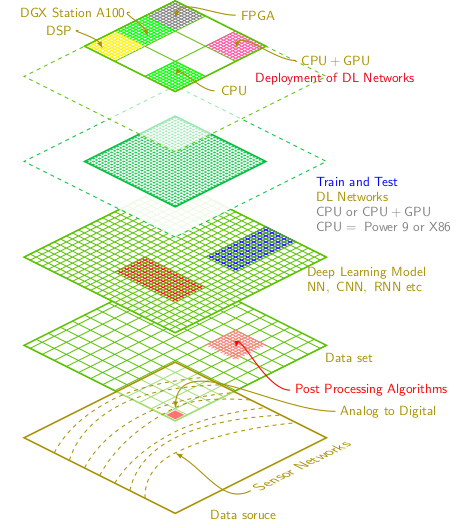
\includegraphics[scale=0.36]{pic/Layers.png}
\caption{ Architecture in DL Product Development }
\label{Layer1}
\end{figure}
\end{frame}

\begin{frame}
\begin{block}{Define model elements  }
Define specialized model element types based on components, ports, and connectors. 
\end{block}
\end{frame}


\begin{frame}
\frametitle{System Architecture Modeling }
\begin{block}{Stereotypes to extend the architectural}
\begin{enumerate}
 \setlength{\itemsep}{0pt}
    \item  Specify interfaces on ports to represent information exchange between components.
    \item    Use stereotypes to extend the architectural modeling language by defining custom metadata for each subsystem or component in the diagram.
\end{enumerate}
\end{block}
\end{frame}





\begin{frame}
\frametitle{Stereotypes  }
\begin{block}{Example}
 A stereotype extends the modeling language with domain-specific metadata. A stereotype adds properties to the root-level architecture, component architecture, ports, connectors, data interfaces, value types, functions, requirements, and requirement links. 

 \url{https://in.mathworks.com/help/systemcomposer/gs/extend-architectural-design.html}
 
\end{block}
\end{frame}

\begin{frame}
\begin{block}{Define Stereotypes }
Define a profile containing a set of stereotypes that describe some analyzable properties (for example, cost and weight).

Define Profiles and Stereotypes 
\url{https://in.mathworks.com/help/systemcomposer/ug/customize-model-elements.html}


\end{block}
\end{frame}



\begin{frame}
\frametitle{System Architecture Modeling }
\begin{block}{ Model Allocations}
\begin{enumerate}
 \setlength{\itemsep}{0pt}
      \item   First, define profiles with stereotypes, then apply stereotypes to model elements, and finally assign unique property values to describe each element. 
    \item  Establish traceability using requirements management and model-to-model allocations Compose Architectures Visually (System Composer)  
\end{enumerate}

\url{https://in.mathworks.com/help/systemcomposer/ug/author-composition.html}

\end{block}
\end{frame}



\begin{frame}
\frametitle{System Composer architecture }
\begin{block}{Visualize }
\begin{enumerate}
 \setlength{\itemsep}{0pt}
      \item    A System Composer architecture represents a system of components and how they interface with each other structurally and behaviorally.
    \item   Different types of architectures describe different aspects of systems. You can use views to visualize a subset of components in an architecture. 
\end{enumerate}
\end{block}
\end{frame}



\begin{frame}
\frametitle{Sub System Interconnect }
\begin{figure}
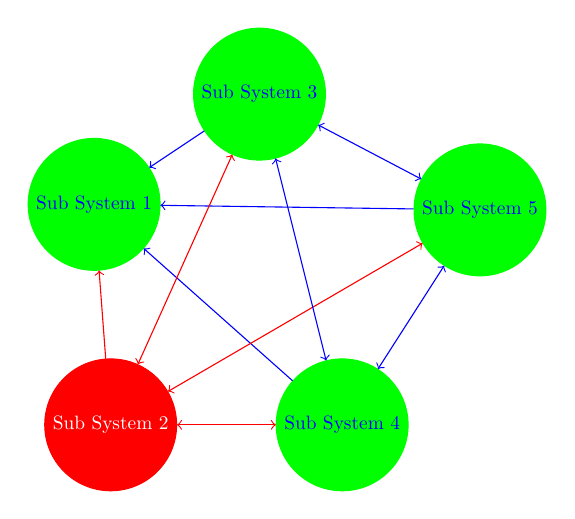
\begin{tikzpicture}[scale=0.7,transform shape,every state/.style={minimum width={1cm},thick,align=center},state/.style={circle, draw, minimum size=1cm}]
\node[state] [color=green, fill=green] (1) {{\color{blue}  Sub System 1}};
\node[state] [color=green, fill=green]  at (3, 2) (3) {
{\color{blue} Sub  System 3}   };
\node[state] [color=green, fill=green] at (7, -0.1) (5) {{\color{blue}  Sub System 5}};
\node[state] [color=red, fill=red] at (0.3,-4) (2) {{\color{white}  Sub System 2}};
\node[state] [color=green, fill=green] at (4.5,-4) (4) {{\color{blue}  Sub System 4}};
					
					\draw[<-] [draw = red](1) -- node [ midway,above] {} (2);
					\draw[<-] [draw = blue] (1) -- node [midway,below] {} (3);
					\draw[<-] [draw = blue] (1) -- node [midway,below] {} (4);
					\draw[<-] [draw = blue] (1) -- node [midway,below] {} (5);
					
					\draw[<->] [draw = red] (2) -- node [midway,below] {} (3);
					\draw[<->] [draw = red] (2) -- node [midway,below] {} (4);
					\draw[<->] [draw = red] (2) -- node [midway,below] {} (5);
					
					\draw[<->] [draw = blue] (3) -- node [midway,below] {} (4);
					\draw[<->] [draw = blue] (3) -- node [midway,below] {} (5);
					
					\draw[<->] [draw = blue] (4) -- node [midway,below] {} (5);
				\end{tikzpicture}
		
\caption{Red is faulty sensor, Green is good sensor}
\label{rgpic}
\end{figure}
\end{frame}





\begin{frame}
\frametitle{System Composer architecture }
\begin{block}{ Architectural information }
\begin{enumerate}
 \setlength{\itemsep}{0pt}
      \item      User can define parameters on the architecture level using the Parameter Editor.
    \item   A System Composer model is the file that contains architectural information, including components, ports, connectors, interfaces, and behaviors. 
\end{enumerate}

\end{block}
\end{frame}

\begin{frame}
\frametitle{Hidden Layer in Architecture }
\begin{figure}
\includegraphics[scale=0.7]{pic/network2.PNG}
\caption{ Layers in Architecture }
\label{Layer1}
\end{figure}
\end{frame}

\begin{frame}
\frametitle{System Composer architecture }
\begin{block}{ Top-level  }
\begin{enumerate}
 \setlength{\itemsep}{0pt}
      \item    An architecture model includes a top-level architecture that holds the composition of the system. 
    \item    This top-level architecture also allows definition of interfaces of this system with other systems.
\end{enumerate}
\end{block}
\end{frame}


\begin{frame}
\frametitle{System Composer architecture }
\begin{block}{ How to }
\begin{enumerate}
 \setlength{\itemsep}{0pt}
      \item     Start with a blank architecture model to model the physical and logical architecture of a system.
\end{enumerate}

\end{block}
\end{frame}









\begin{frame}
\begin{block}{Architecture for Model Based Systems}
 Model-Based Systems Engineering for Space-Based Applications 
 
\url{https://in.mathworks.com/help/systemcomposer/ug/model-based-systems-engineering-space-based-applications.html}
\end{block}
\end{frame}

\begin{frame}
\begin{block}{Define the connections to Interact with Model }
Learn about port interfaces that define the connections between components. \\
\url{https://in.mathworks.com/help/systemcomposer/ug/define-port-interfaces-between-components.html}
\end{block}
\end{frame}



\begin{frame}
\begin{block}{Space mission architecture }

\begin{enumerate}
    \item  Simulink
    \item  System Composer
\end{enumerate}

 CubeSat Model-Based System Engineering Project template, available from the Simulink® start page, under Aerospace Blockset™. 
 
 It demonstrates how to model a space mission architecture in Simulink with System Composer™ and Aerospace Blockset for a 1U CubeSat in low Earth orbit (LEO). The CubeSat's mission is to image MathWorks Headquarters in Natick, Massachusetts at least once per day. The project references the Aerospace Blockset CubeSat Simulation Project, reusing the vehicle dynamics, environment models, data dictionaries, and flight control system models defined in that project.
\end{block}
\end{frame}


\begin{frame}
\begin{block}{ CubeSat Model-Based System}
 how to model a space mission architecture in Simulink with System Composer™ and Aerospace Blockset for a 1U CubeSat in low Earth orbit (LEO).  
\end{block}
\end{frame}

\begin{frame}
\begin{block}{ CubeSatmission}
  The CubeSat's mission is to image MathWorks Headquarters in Natick, Massachusetts at least once per day.  
\end{block}
\end{frame}

\begin{frame}
\begin{block}{ Reuse, Reduce Cost}
 Project references the Aerospace Blockset CubeSat Simulation Project, reusing the vehicle dynamics, environment models, data dictionaries, and flight control system models defined in that project.
\end{block}
\end{frame}


\begin{frame}
\begin{block}{Define system level requirements}
For a CubeSat mission in Simulink Compose a system architecture

  for the mission in System Composer Link system-level requirements to components in the architecture with Requirements Toolbox™ Model vehicle dynamics and flight control systems with Aerospace Blockset Validate orbital requirements using mission analysis tools and Simulink Test™
\end{block}
\end{frame}

\begin{frame}
\begin{block}{Analyze Architecture }


\url{ https://in.mathworks.com/help/systemcomposer/ug/analyze-architecture.html}


 Perform static analysis on a System Composer™ architecture to evaluate characteristics of the system.

Analysis is a method for quantitatively evaluating an architecture for certain characteristics. Static analysis analyzes the structure of the system. Static analysis uses an analysis function and parametric values of properties captured in the system model.

Use analyses to calculate overall reliability, mass roll-up, performance, or thermal characteristics of a system, or to perform a SWaP analysis.



\end{block}
\end{frame}



\begin{frame}
\begin{block}{Quantitatively evaluating Step }

Analysis is a method for quantitatively evaluating an architecture for certain characteristics. Static analysis analyzes the structure of the system. Static analysis uses an analysis function and parametric values of properties captured in the system model.

Use analyses to calculate overall reliability, mass roll-up, performance, or thermal characteristics of a system, or to perform a SWaP analysis.
\end{block}
\end{frame}



\begin{frame}
\begin{block}{Static analyses}
Write static analyses based on element properties to perform data-driven trade studies and verify system requirements. Consider an electro mechanical system where there is a trade-off between cost and weight, and lighter components tend to cost more.

\end{block}
\end{frame}

\begin{frame}
\begin{block}{Decision process}

Decision process involves analyzing the overall cost and weight of the system based on the properties of its elements, and iterating on the properties to arrive at a solution that is acceptable both from the cost and weight perspective.
\end{block}
\end{frame}


\begin{frame}
\begin{block}{Profile to an architecture model }
Apply the profile to an architecture model and add stereotypes from that profile to elements of the model (components, ports, or connectors).

Specify values for the properties on those elements.

Write an analysis function to compute values necessary for the trade study. This is a static constraint solver for parametric and values of related properties captured in the system model.
\end{block}
\end{frame}



\begin{frame}
\begin{block}{Instance architecture model }

Create an instance of the architecture model, which is a tree of elements, corresponding to the model hierarchy with all shared architectures expanded and a variant configuration applied. Use the Instantiate Architecture Model tool.

Run the analysis function and then see analysis calculations and results in the Analysis Viewer tool.

\end{block}
\end{frame}



\begin{frame}
\begin{block}{Brain Tech Talk }

\url{https://youtu.be/pSfZutP9H-U}

architecture \\
\url{https://youtu.be/UTm1ORuZ1dg}

\end{block}
\end{frame}

